\documentclass[preview]{standalone}

\usepackage{amsmath}
\usepackage{amssymb}
\usepackage{tikz}
\usepackage{stellar}
\usepackage{bettelini}

\hypersetup{
    colorlinks=true,
    linkcolor=black,
    urlcolor=blue,
    pdftitle={Stellar},
    pdfpagemode=FullScreen,
}

\begin{document}

\id{geofisica-moticonvettivi}
\genpage

\section{Moti convettivi}

\begin{snippetdefinition}{moto-convettivo}{Moto convettivo}
    I \textit{moti convettivi} sono dei lenti movimenti di materiali solidi.
\end{snippetdefinition}

\begin{snippet}{8b662878-bf7f-4c41-84ab-f6c717e69a6c}
    I moti convettivi possono scendere o salire.
    Quando i moti salgono e colpiscono la litosfera intaccano le placche tettoniche.
    
    Le zolle litosferico sono strutture rigide che galleggiano sulla sottostante astenosfera,
    la quale funge da strato plastico entro il quale si realizzano moti convettivi.
    
    Le zolle litosferiche possono essere composte da litosfera continentale o litosfera oceanica
    (con crosta continentale e crosta oceanica) oppure entrambe.
\end{snippet}

\section{Litosfera e movimento delle placche}

\begin{snippet}{litosfera-composizione-expl}
    La litosfera è suddivisa in placche di dimensioni variabili, che si incastrano tra loro come
    tessere di un mosaico, senza lasciare spazi vuoti. Le placche litosferiche sono rigide, hanno
    uno spessore variabile e si muovono sull'astenosfera, che si comporta come uno strato plastico.
    In questo strato, si verificano lenti movimenti di materiale con correnti ascensionali e
    discensionali, noti come movimenti convettivi.
\end{snippet}

\begin{snippet}{litosfera-placche-illustration}
    \begin{figure*}[ht!]
        \begin{center}
            \begin{tikzpicture}
                \node[anchor=south west,inner sep=0] (image) at (0,0) {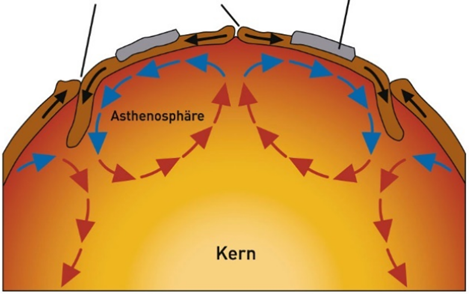
\includegraphics[width=0.4\textwidth]{resources/placche-tettoniche.png}};
                \node at (.4,4.5) {\footnotesize Attività sismiche};
                \node at (3.3,4.5) {\footnotesize Fenomeni magmatici};
                \node at (5.7,4.5) {\footnotesize Continenti};
            \end{tikzpicture}
        \end{center}
    \end{figure*}
\end{snippet}

\begin{snippet}{movimento-placche-expl}
    Le placche si muovono orizzontalmente. Poiché sono a diretto contatto tra loro, ogni movimento
    di una placca influenza quelli delle placche vicine. Questo genera instabilità lungo i margini
    delle placche, mentre le regioni centrali di ciascuna placca sono sostanzialmente inattive e
    stabili. Questo fenomeno permette di identificare i margini delle placche, che corrispondono a
    fasce sottili e allungate caratterizzate da attività sismica.
\end{snippet}

\end{document}